\documentclass{report}

\usepackage{amsmath}
\usepackage{graphicx} % to insert images
\usepackage{array} % Included to solve invalid char in Tables declaration
\usepackage[margin=1in]{geometry} % sets page margins
\usepackage{graphicx} % to insert images
\graphicspath{{../pdf/}{/Users/rutviksayankar/Repos/ECE483_FinalProject/Simulations/Graphs}} % setting up path for image storage
\usepackage{hyperref} % allows table of contents to be clickable to sections
\hypersetup{
    colorlinks,
    citecolor=blue,
    filecolor=blue,
    linkcolor=blue,
    urlcolor=blue
}

% This section redefines the chapter headings, this allows us to remove the implicit "Chapter #" that comes before a provided chapter title.
\makeatletter
\def\@makechapterhead#1{%
  \vspace*{20\p@}%
  {\parindent \z@ \raggedright \normalfont
    \ifnum \c@secnumdepth >\m@ne
      %\if@mainmatter
        %\huge\bfseries \@chapapp\space \thechapter
        \Huge\bfseries \thechapter.\space%
        %\par\nobreak
        %\vskip 20\p@
      %\fi
    \fi
    \interlinepenalty\@M
    \Huge \bfseries #1\par\nobreak
    \vskip 40\p@
  }}
\makeatother

\title{ECE 483: Analog IC Design \\ Final Report \\ Low Dropout Regulator} % Sets article title

\author {
    \textbf{Sayankar, Rutvik}\\
    \textit{rutviks2@illinois.edu} \\
    \hfill \\ 
    \textbf{Patel, Dev}\\
    \textit{dpatel2@illinois.edu} \\
    \hfill \\ 
} 
\date{\today} % Sets date for date compiled

% The preamble ends with the command \begin{document}
\begin{document}
    \maketitle % creates title using information in preamble (title, author, date)
    
    \pagebreak


    \chapter{Overall Design Approach}
    \section{Design choices}
    asdf

    \section{System level trade-offs}
    asdf

    \chapter{Schematic \& Parameters}
    \section{Schematic}


    \section{Device Parameters}
    \begin{center}
        \begin{tabular}{|m{4em}|m{3em}|m{3em}| m{4em}| m{4em}| m{4em}| m{4em} |m{4em} |}
            \hline
            Device & W($\mu$m) & L(nm) & Multiplier & $g_m$($\mu$S) & $r_{ds}$(ohms) & Vov(mV) & $I_{bias}$ ($\mu$A) \\
            \hline
            MPass & 1.08 & 270 & 500 & 12.41m & 5.864k & 106.1 & 800
            \\
            \hline
            MP0 & 1.44 & 270 & 24 & 881.1 & 23.07k & 114.7 & 60
            \\
            \hline
            MP1 & 1.44 & 270 & 24 & 911.2 & 770.3k & 108.5 & 59.99
            \\
            \hline
            MP2 & 1.44 & 270 & 24 & 552.5 & 161.7k & 57.96 & 29.96
            \\
            \hline
            Mp3 & 1.44 & 270 & 24 & 552 & 161.9k & 58.41 & 29.97
            \\
            \hline
            MP4 & 1.44 & 270 & 4 & 148.7 & 132.3k & 116.1 & 10.2
            \\
            \hline
            MP5 & 1.44 & 270 & 4 & 154 & 466.9k & 109.5 & 10.2
            \\
            \hline
            MP6 & 1.44 & 270 & 4 & 148,7 & 131.9k & 116.1 & 10.19
            \\
            \hline
            MP7 & 1.44 & 270 & 4 & 153.9 & 459.8k & 109.6 & 10.19
            \\
            \hline
            MP8 & 1.44 & 270 & 4 & 147.6 & 148.5k & 114.7 & 10.03
            \\
            \hline
            MP9 & 1.44 & 270 & 4 & 153 & 562.2k & 104.2 & 10.03
            \\
            \hline
            MP10 & 1.44 & 270 & 4 & 147 & 139k & 114.7 & 10
            \\
            \hline
            MP11 & 1.44 & 270 & 4 & 152 & 473.1k & 108.2 & 10
            \\
            \hline
            MN0 & .72 & 540 & 6 & 174.5 & 596.1k & 89.27 & 10.2
            \\
            \hline
            MN2 & .72 & 540 & 8 & 444 & 69.14k & 177.1 & 40.17
            \\
            \hline
            MN4 & .72 & 540 & 6 & 172 & 511.6k & 90.43 & 10.03
            \\
            \hline
            MN5 & .72 & 540 & 2 & 110.7 & 263.9k & 177.1 & 10.03
            \\
            \hline
            MN6 & .72 & 540 & 6 & 174.5 & 596.7k & 89.22 & 10.19
            \\
            \hline
            MN7 & .72 & 540 & 8 & 444.1 & 69.22k & 177.1 & 40.17
            \\
            \hline
        \end{tabular}
    \end{center}
    
        

    \chapter{Performance}

    \section{Simulation Results}
    \begin{center}
        \begin{tabular}{|m{25em}|m{7em}|m{12em}|}
            \hline
            \textbf{Design Parameter/Variable} & \textbf{Specification} & \textbf{Simulated Performance} \\
            \hline
            \hline
            Input Voltage & 1.8V $\pm$ 10$\%$ & 1.8V \\
            \hline
            Output Voltage & 1.0V - 1.4V  & 1.0V - 1.4V \\
            \hline
            Load Current & 0.1mA - 10mA & 0.1mA - 10mA \\
            \hline
            DC Load Regulation & $\leq$ 50$\mu$V/mA & 15.55$\mu$V/mA\\
            \hline
            DC Line Regulation & $\leq$ 500$\mu$V/V & 750$\mu$V/V\\
            \hline
            Quiescent Current & Minimum & 600$\mu$A \\
            \hline
            PSR (@Fin = 1KHz/Fin = 1MHz) & - & -72.97dB/-12.31dB\\
            \hline
            Worst-case PSR & - & -1.42dB\\
            \hline
            DC loop gain (IL=0.1mA/IL=10mA) & - & 86.22 dB / 75.64 dB\\
            \hline
            Loop-gain unity-gain frequency (IL=0.1mA/IL=10mA) & - & 3.981 MHz / 3.479 MHz\\
            \hline
            Loop-gain phase margin(IL=0.1mA/IL=10mA) & - & 62.4$^{\circ}$ / 82.35$^{\circ}$  \\
            \hline
            Loop-gain gain margin (IL=0.1mA/IL=10mA) & - & 23.61 dB / 28.72 dB \\ 
            \hline
            Output noise (IL=0.1mA/IL=10mA) & - & $61.3\mu V$ / $58.1 \mu V$\\
            \hline

            \end{tabular}
    \end{center}

    \subsection{Loop-gain AC response}
    \begin{figure}[ht!]
        \centering
        \begin{minipage}[b]{0.4\linewidth}
            \centering
            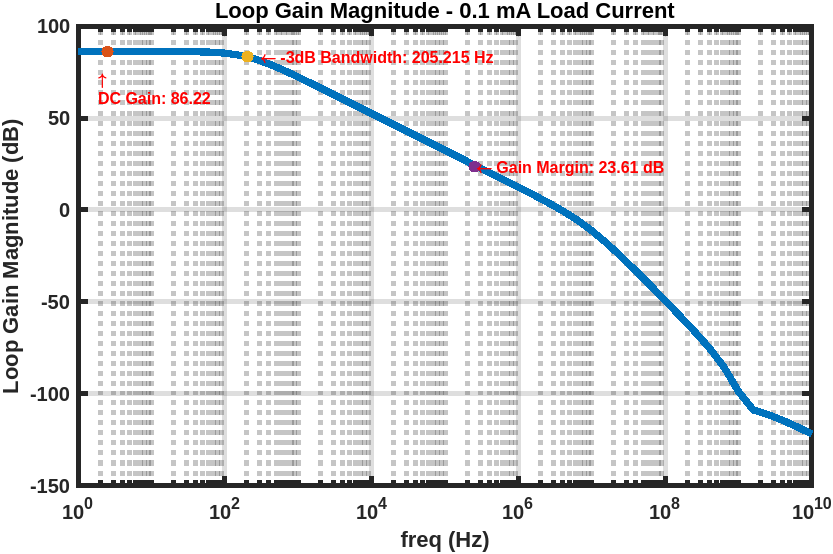
\includegraphics[width=\linewidth]{LoopGainMagnitudeMinLoadCurrent.png}
            % \caption{LG Magnitude at 0.1mA}
            \label{fig:LoopGainMagnitudeMinLoadCurrent}
        \end{minipage}
        \begin{minipage}[b]{0.4\linewidth}
            \centering
            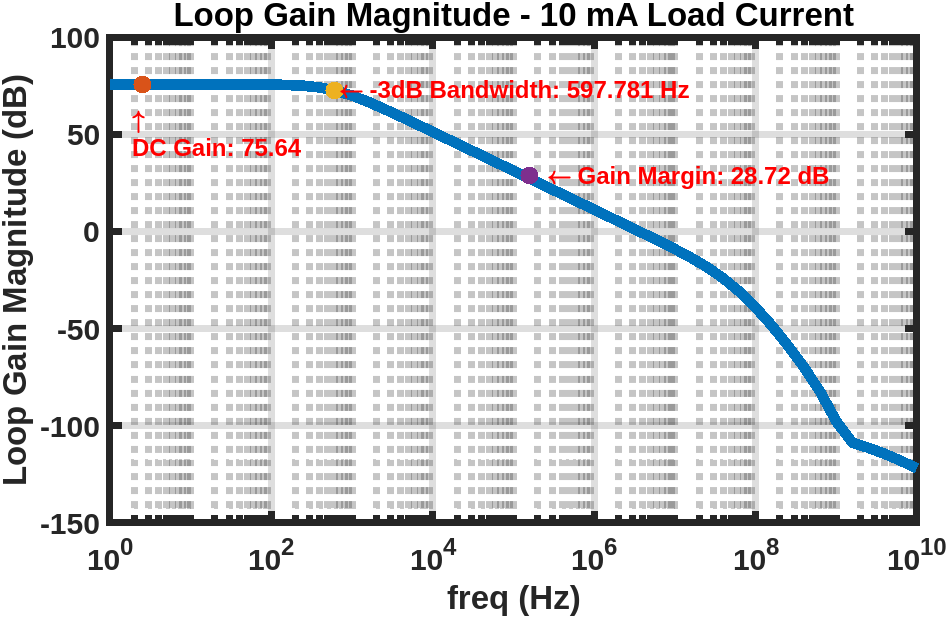
\includegraphics[width=\linewidth]{LoopGainMagnitudeMaxLoadCurrent.png}
            % \caption{LG Magnitude at 10mA}
            \label{fig:LoopGainMagnitudeMaxLoadCurrent}
        \end{minipage}
        \hfill
        \begin{minipage}[b]{0.4\linewidth}
            \centering
            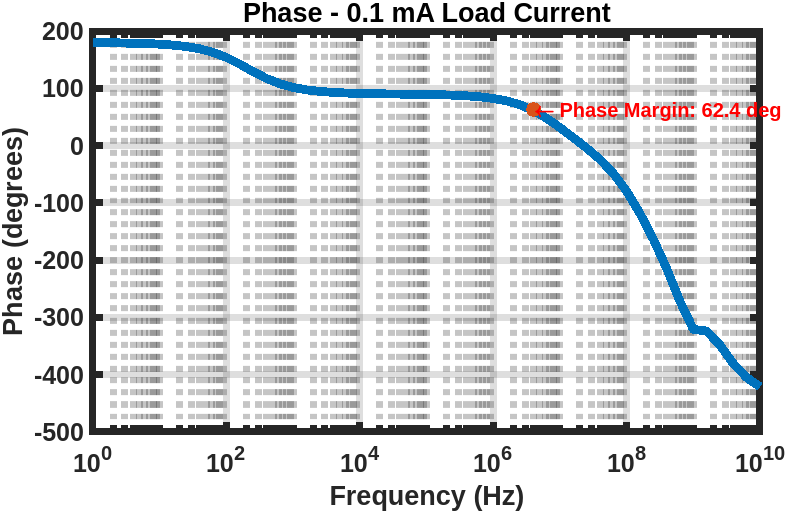
\includegraphics[width=\linewidth]{LoopGainPhaseMinLoadCurrent.png}
            % \caption{LG Phase at 0.1mA}
            \label{fig:LoopGainPhaseMinLoadCurrent}
        \end{minipage}
        \begin{minipage}[b]{0.4\linewidth}
            \centering
            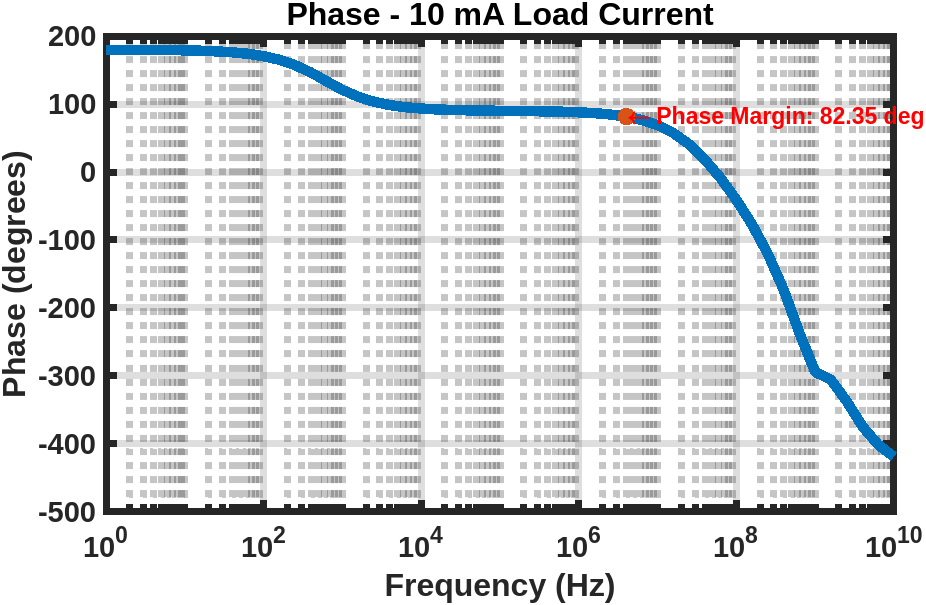
\includegraphics[width=\linewidth]{LoopGainPhaseMaxLoadCurrent.png}
            % \caption{LG Phase at 10mA}
            \label{fig:LoopGainPhaseMaxLoadCurrent}
        \end{minipage}
    \end{figure}

    \pagebreak

    \subsection{DC load and line regulation response}

    \begin{center}
        \begin{tabular}{lll}
            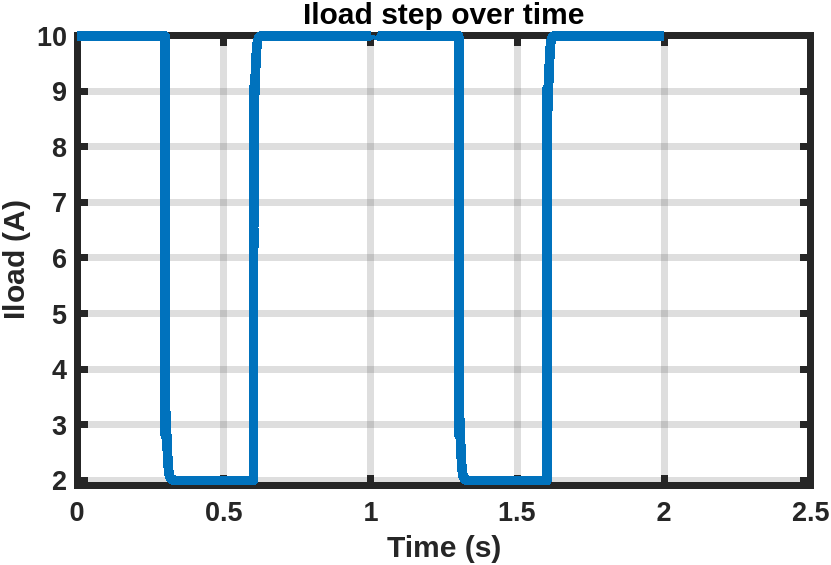
\includegraphics[width=0.3\linewidth]{IloadStep.png} & 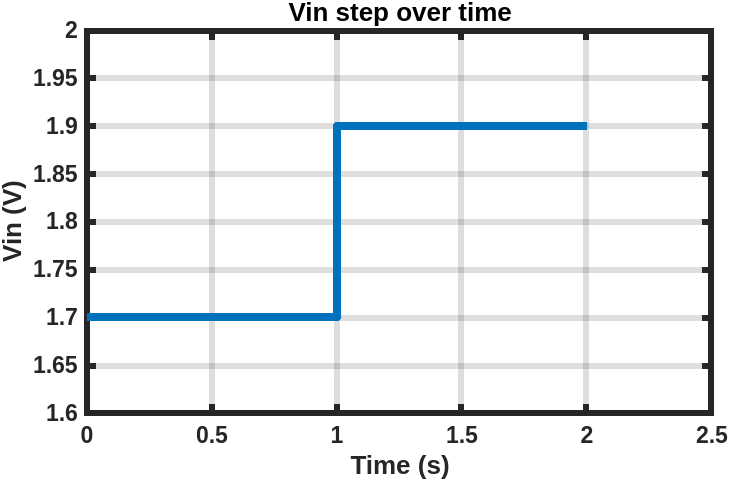
\includegraphics[width=0.3\linewidth]{VinStep.png} & 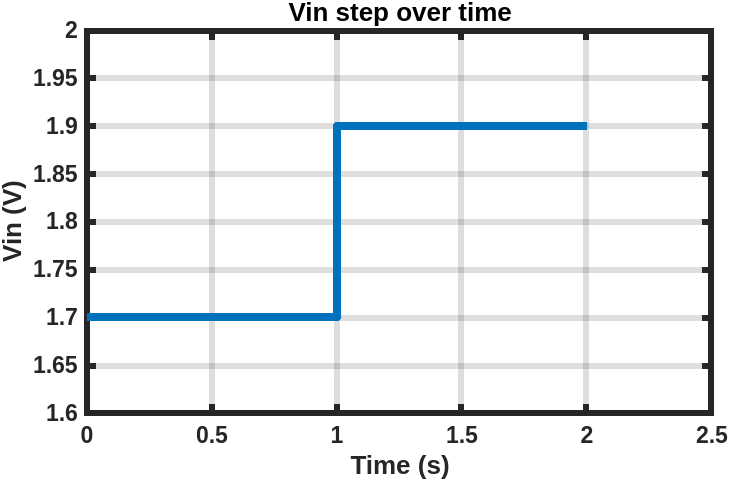
\includegraphics[width=0.3\linewidth]{VinStep.png}\\
            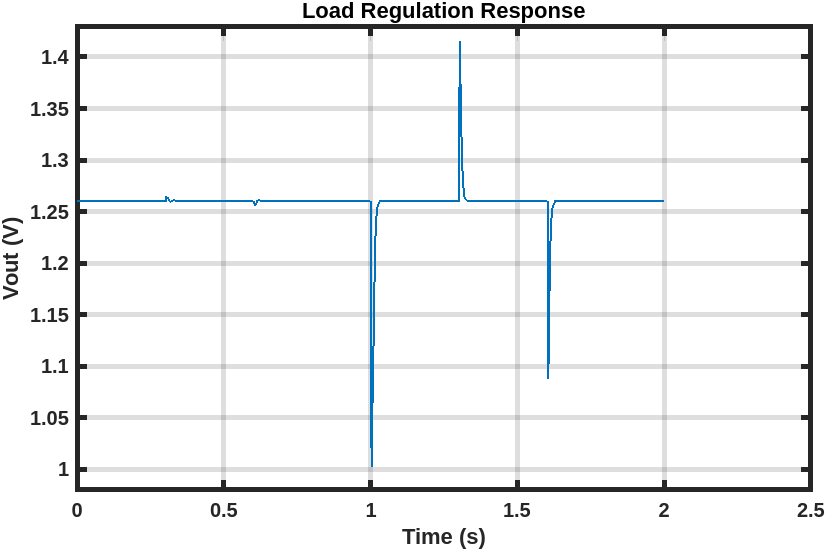
\includegraphics[width=0.3\linewidth]{LoadReg.png} & 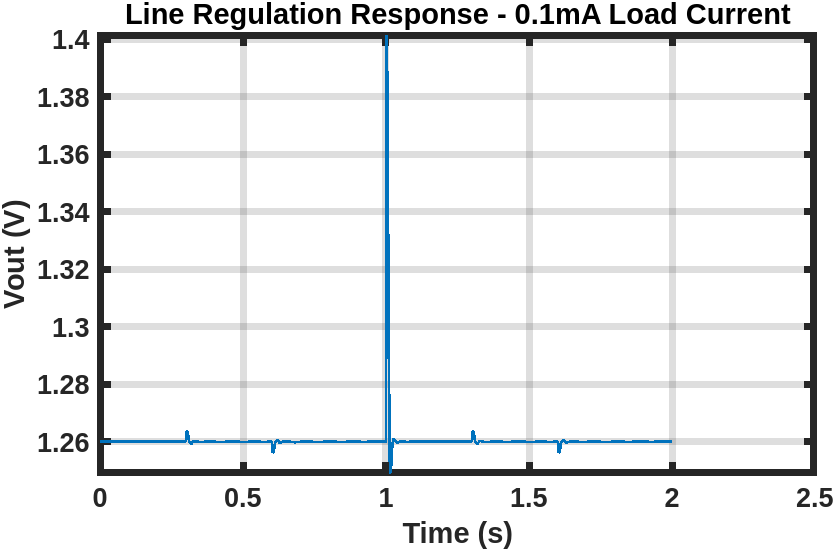
\includegraphics[width=0.3\linewidth]{LineRegMinLoadCurrent.png} & 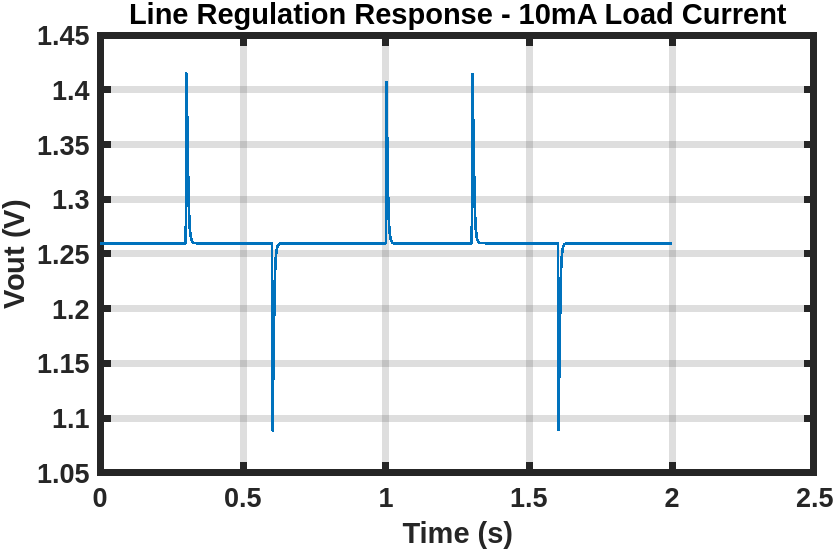
\includegraphics[width=0.3\linewidth]{LineRegMaxLoadCurrent.png}\\
        \end{tabular}
    \end{center}


    \subsection{Power supply rejection (PSR)}

    \begin{figure}[ht!]
        \centering
        \begin{minipage}[b]{0.45\linewidth}
            \centering
            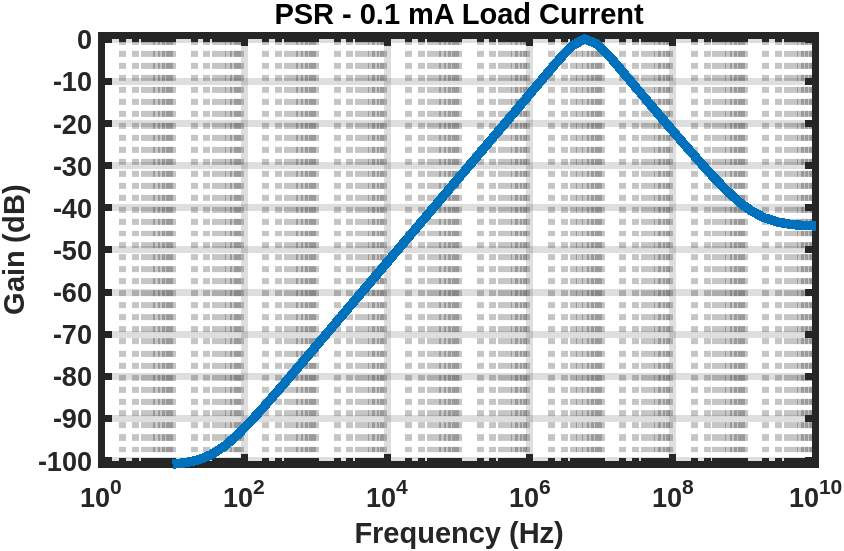
\includegraphics[width=\linewidth]{PSRMinLoadCurrent.png}
            \caption{PSR with Minimum Load Current}
            \label{fig:PSRMinLoadCurrent}
        \end{minipage}
        \hfill
        \begin{minipage}[b]{0.45\linewidth}
            \centering
            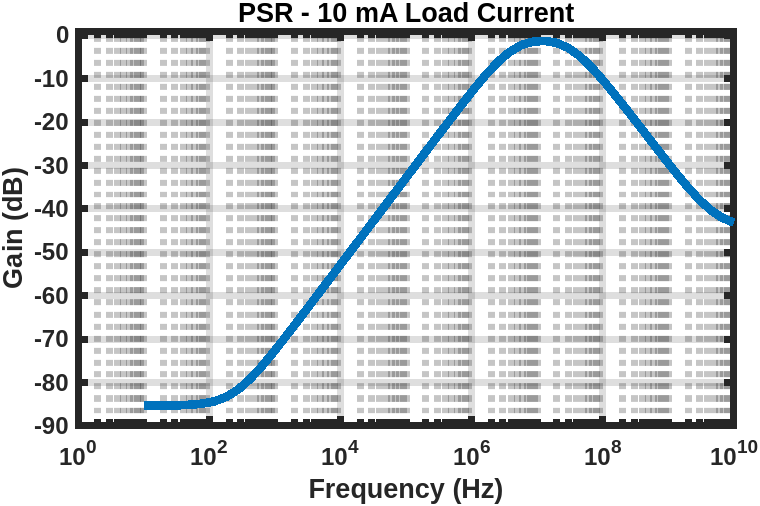
\includegraphics[width=\linewidth]{PSRMaxLoadCurrent.png}
            \caption{PSR with Maximum Load Current}
            \label{fig:PSRMaxLoadCurrent}
        \end{minipage}
    \end{figure}

\end{document} % This is the end of the document